\section{General setup}\label{sec:general-setup}
GROOVE has several exploration strategies for exploring a GG. The SymbolicStrategy is added as exploration strategy. It contains functionality to build an IOSTS from an IOGG. Figure~\ref{fig:tooling} shows the UML sequence diagram of GRATiS. The functionality of GROOVE and ATM as described in Figures~\ref{fig:axini_tool} and \ref{fig:groove_tool} is omitted where possible.

\begin{figure}[ht]
  \begin{center}
    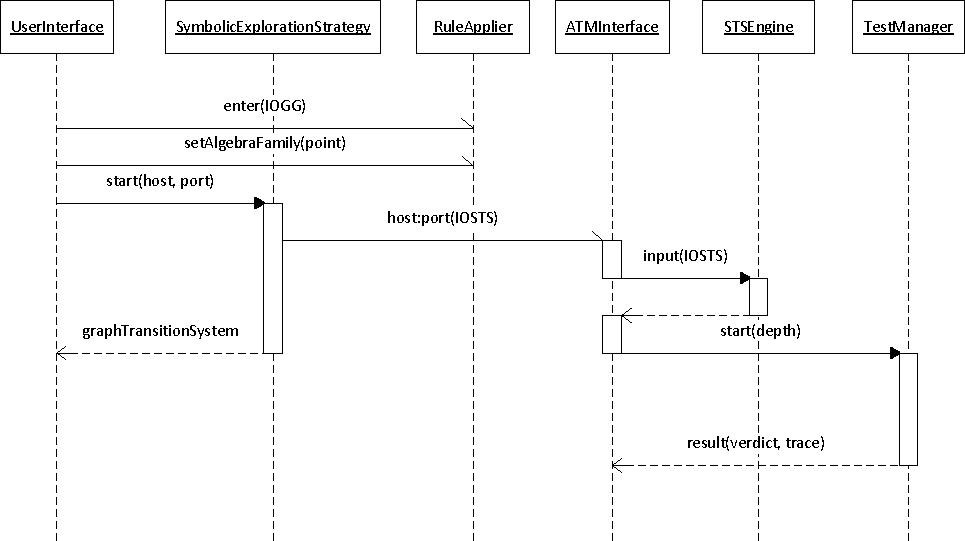
\includegraphics[width=\textwidth]{gratis_diagram.pdf}
  \end{center}
  \caption{GRATiS sequence diagram}
  \label{fig:tooling}
\end{figure}

\begin{enumerate}
\item The user enters an IOGG in the RuleApplier.
\item The user sets the algebra family of the IOGG to to the point algebra. 
\item The user starts the SymbolicExplorationStrategy with a host and port. The communication between the RuleApplier and the strategy is omitted here. However, it should be noted that the point algebra is used by the RuleApplier here to create the rule transitions.
\item The SymbolicExplorationStrategy creates an IOSTS from the IOGTS and sends the IOSTS to the given host and port.
\item The IOSTS is given to the STSEngine. The ATMInterface takes the role of the UserInterface in ATM.
\item The ATMInterface starts the testing using a configurable depth parameter. The communication between the TestManager, STSEngine and Adapter is omitted here.
\item The TestManager returns the test results. The test results are stored in a database and are viewable through the user interface of ATM.
\end{enumerate}

\section{Description of added functionality}
This section covers in detail the added functionality to GROOVE and ATM. 

\subsection{GROOVE exploration strategy}
Figure~\ref{fig:esi-diagram} shows the class diagram of the added exploration strategy interface. The SymbolicExplorationStrategy has an exploration strategy such as the BreadthFirstStrategy to explore the GTS. The remote exploration strategy extends the symbolic exploration strategy.

The user starts the remote exploration strategy with a host and port. This strategy starts a breadth-first exploration strategy. This strategy explores the IOGG and notifies the remote strategy when there are no more rule transitions to explore. The symbolic strategy builds the IOSTS in Java objects using the explored rule transitions. The class diagram  of the IOSTS is given in section~\ref{sec:sts-setup}. The remote strategy sends the IOSTS in JSON format as a HTTP POST request to the interface at ATM.

The breadth-first exploration strategy and the symbolic strategy are loosely coupled, such that other strategies can also be used if desired.
 
\begin{figure}[ht]
  \begin{center}
    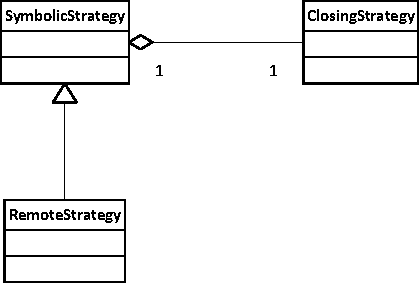
\includegraphics[width=0.35\textwidth]{strategy.pdf}
  \end{center}
  \caption{The class diagram of the exploration strategy interface}
  \label{fig:esi-diagram}
\end{figure}

\subsection{STSs}\label{sec:sts-setup}
Figure~\ref{fig:sts-diagram} shows the class diagram of the IOSTS in GRATiS. The IOSTS is composed of Location, SwitchRelation, Gate, Interaction- and LocationVariable classes. A Location object can be the start and target of any number of SwitchRelation objects. A SwitchRelation object has two Location objects; the start and target location. It also has one Gate object, which can belong to any number of SwitchRelation objects. A Gate object can have any number of InteractionVariable objects, but an InteractionVariable object belongs to only one Gate object. The IOSTS has a singleton class, the RuleInspector, which contains the functionality of building guards and updates from rule graphs.

\begin{figure}[ht]
  \begin{center}
    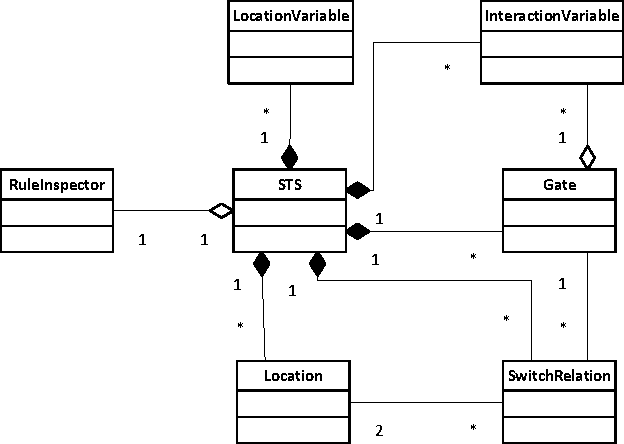
\includegraphics[width=0.5\textwidth]{STS.pdf}
  \end{center}
  \caption{The class diagram of the IOSTS in GRATiS}
  \label{fig:sts-diagram}
\end{figure}

Figure~\ref{fig:sts-objects} shows the object relations in accordance with the class diagram for the IOSTS in Figure~\ref{fig:example_sts}. Note that the links between the $\mathit{BoardGame}$ object and the Location, SwitchRelation, IOGate and InteractionVariable classes are not drawn for the sake of clarity.

\begin{figure}[ht]
  \begin{center}
    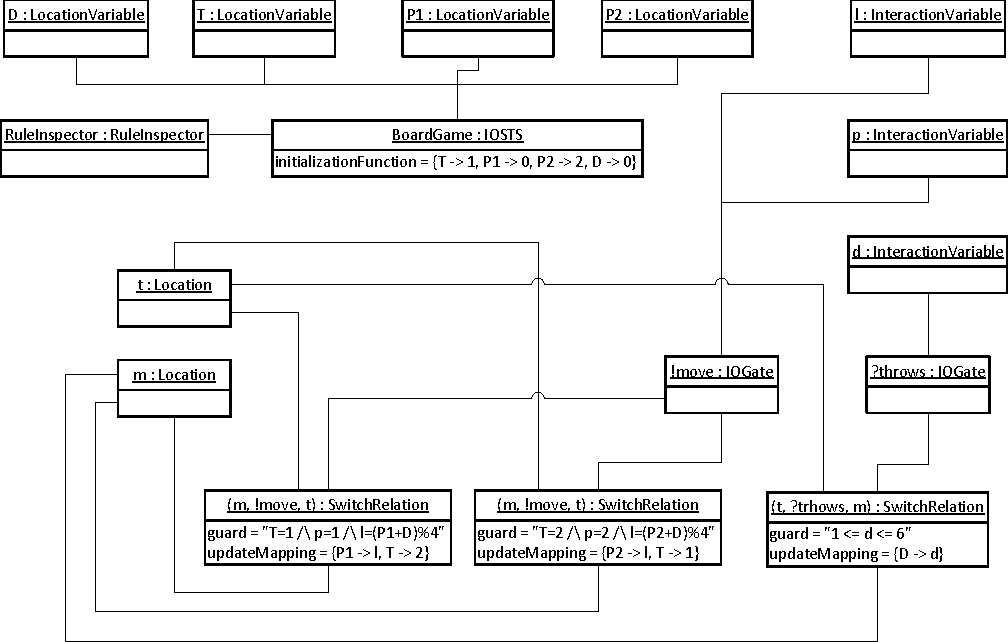
\includegraphics[width=0.8\textwidth]{STS_objects.pdf}
  \end{center}
  \caption{The object diagram of the IOSTS in Figure~\ref{fig:example_sts}}
  \label{fig:sts-objects}
\end{figure}

\subsection{ATM Interface}
The ATM interface is one component in the Ruby on Rails framework. The interface is a controller in this Model-View-Controller framework. Controllers handle the HTTP requests given by the framework. The interface receives the IOSTS POST request, builds the IOSTS as Ruby objects and initiates the test using this IOSTS as model.